\section{Results}\label{sec:results}
The results for exercises 1, 2, and 3 are briefly presented in the following sections.

\subsection{Exercise 1}\label{subsec:exercise_1}
For exercise 1, the Runge-Kutta method was implemented using the Butcher Tableau. As a result, the approximated value for the ordinary differential equation is obtained for each time step. The results are displayed in Table \ref{tab:results_ex1}.
\begin{table}[htb!]
    \centering
    \caption{Results for the Runge-Kutta method}
    \begin{tabular}{cc}
        \toprule
        $x$ & $y$ \\
        \midrule
        2.0 & 1.0 \\
        2.1 & 1.19091 \\
        2.2 & 1.36667 \\
        2.3 & 1.53077 \\
        2.4 & 1.68571 \\
        2.5 & 1.83333 \\
        2.6 & 1.97500 \\
        2.7 & 2.11176 \\
        2.8 & 2.24444 \\
        2.9 & 2.37368 \\
        3.0 & 2.50000 \\
        \bottomrule
    \end{tabular}
    \label{tab:results_ex1}
\end{table}

\subsection{Exercise 2}\label{subsec:exercise_2}
For exercise 2, Table
\ref{tab:results_ex2} presents the $\alpha_i$ coefficients for the approximation of $u_h$ depending on the polynomial order $n$. 
\begin{table}[htb!]
    \centering
    \caption{Results for the approximation of $u_h$}
    \begin{tabular}{cccccc}
        \hline
        $\bm{\alpha}$ & $n=1$ & $n=2$ & $n=3$ & $n=4$ & $n=5$ \\ \hline
        $\alpha_1$ & -4.33e-9 & 0.6320 & 0.4918 & 0.4927 & 0.4981 \\
        $\alpha_2$ & - & -0.6108 & -0.3698 & -0.3713 & -0.3814 \\
        $\alpha_3$ & - & -0.6108 & -0.1215 & -0.1198 & -0.1077 \\
        $\alpha_4$ & - & 0.5685 & -0.3698 & -1.47e-3 & -1.90e-2 \\
        $\alpha_5$ & - & - & 0.2780 & -0.3713 & 1.00e-2 \\ 
        $\alpha_6$ & - & - & 0.0904 & 0.2795 & -0.3814 \\ 
        $\alpha_7$ & - & - & -0.1215 & 9.00e-2 & 0.2922 \\ 
        $\alpha_8$ & - & - & 0.0904 & 1.45e-3 & 8.24e-2 \\ 
        $\alpha_9$ & - & - & 0.03232 & -0.1198 & 1.47e-2 \\
        $\alpha_{10}$ & - & - & - & 9.00e-2 & -7.70e-3 \\
        $\alpha_{11}$ & - & - & - & 2.99e-2 & -0.107 \\
        $\alpha_{12}$ & - & - & - & -1.65e-4 & 8.24e-2 \\
        $\alpha_{13}$ & - & - & - & -1.47e-3 & 2.31e-2 \\
        $\alpha_{14}$ & - & - & - & 1.45e-3 & 4.00e-3 \\
        $\alpha_{15}$ & - & - & - & -1.65e-4 & -2.14e-3 \\
        $\alpha_{16}$ & - & - & - & 1.37e-3 & -1.90e-2 \\
        $\alpha_{17}$ & - & - & - & - & 1.47e-2 \\
        $\alpha_{18}$ & - & - & - & - & 4.00e-3 \\
        $\alpha_{19}$ & - & - & - & - & 9.26e-4 \\
        $\alpha_{20}$ & - & - & - & - & -4.22e-4 \\
        $\alpha_{21}$ & - & - & - & - & 1.00e-2 \\
        $\alpha_{22}$ & - & - & - & - & -7.70e-3 \\
        $\alpha_{23}$ & - & - & - & - & -2.14e-3 \\
        $\alpha_{24}$ & - & - & - & - & -4.22e-4 \\
        $\alpha_{25}$ & - & - & - & - & 4.01e-4 \\\hline
    \end{tabular}
    \label{tab:results_ex2}
\end{table}

Table \ref{tab:error_vs_n} shows the error for the approximation of $u_h$ for each polynomial order $n$, which is also depicted in Figure \ref{fig:error_vs_n}.
\begin{table}
    \centering
    \caption{Error for the approximation of $u_h$ vs. polynomial order $n$}
    \begin{tabular}{cc}
        \toprule
        $n$ & Error \\
        \midrule
        1 & 0.673542425905569 \\
        2 & 0.11149814453502095 \\
        3 & 0.006645639492674947 \\
        4 & 0.006412141835255881 \\
        5 & 0.0021858066887519693 \\
        \bottomrule
    \end{tabular}
    \label{tab:error_vs_n}
\end{table}
\begin{figure}[htb!]
    \centering
    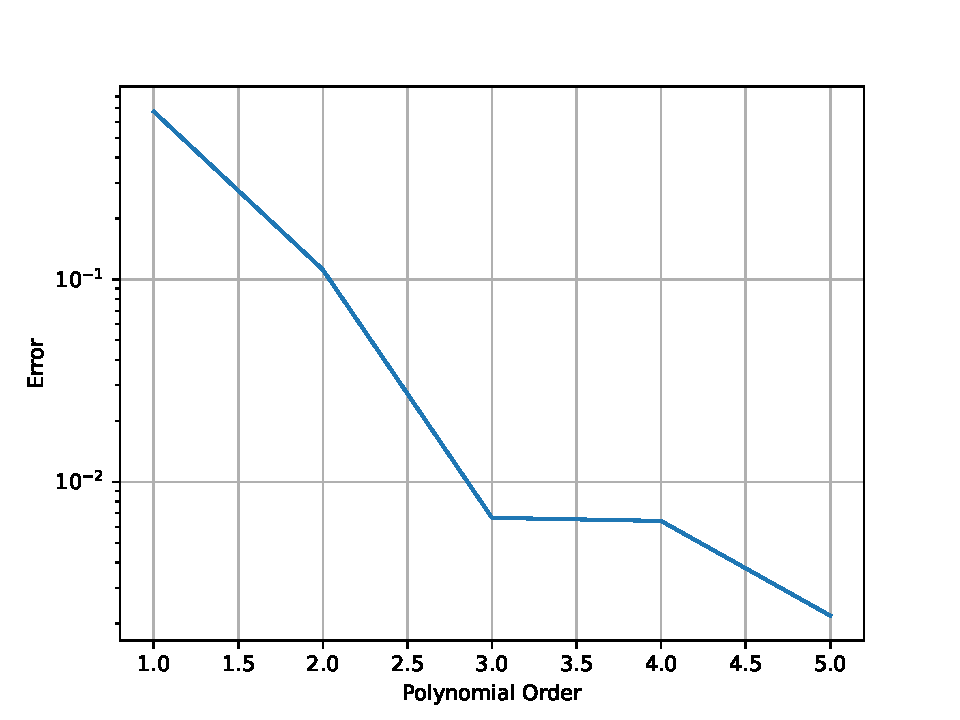
\includegraphics[scale=.9]{Figures/Error_2.pdf}
    \caption{Error for the approximation of $u_h$ vs. polynomial order $n$}
    \label{fig:error_vs_n}
\end{figure}

\subsection{Exercise 3}\label{subsec:exercise_3}
As the main results for exercise 3, the coefficients for the curve fitting (Eq. \eqref{eq:exp_fit}) are presented in Table \ref{tab:results_ex3}, as well as the total error for the approximation.
\begin{table}[htb!]
    \centering
    \caption{Results for the curve fitting}
    \begin{tabular}{ccccc}
        \hline
        \textbf{Approximation Type} & \textbf{Coefficient a} & \textbf{Coefficient b} & \textbf{Curve fitting} & \textbf{Total Error}\\ \hline
        Logarithmic & 0.5974 & 1.2821 & $1.2821x^{0.5974}$ & 24.2828 \\
        Non-linear & 0.5974 & 1.1804 & $1.1804x^{0.5974}$ & 19.7567\\ \hline
    \end{tabular}
    \label{tab:results_ex3}
\end{table}

As expected, the linearization of the logarithmic function provides a worse approximation than the non-linear method, since the latter is the solution of the Least Squares Method. Figure \ref{fig:curve_fitting} shows the data points and the approximated solution for both approximation types.
\begin{figure}[htb!]
    \centering
    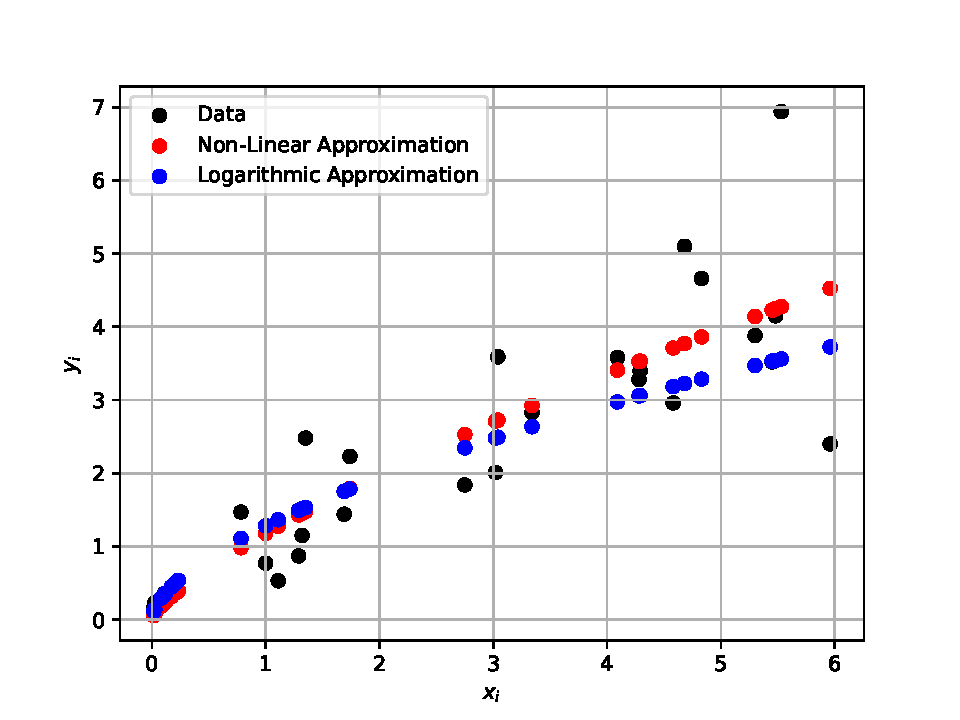
\includegraphics[scale=.9]{Figures/Approx_Comparison.pdf}
    \caption{Curve fitting for the data points using the Least Squares Method}
    \label{fig:curve_fitting}
\end{figure}